%\documentclass[letterpaper, 10 pt, conference]{ieeeconf}  % Comment this line out if you need a4paper
\documentclass[10pt, conference]{IEEEtran}

%Command and package
%Additional Definition
\setlength{\textfloatsep}{3pt plus 1.0pt minus 2.0pt}
\usepackage[ruled, linesnumbered]{algorithm2e}
\usepackage{cite}
\usepackage{mathtools}
\usepackage{geometry}
\usepackage{comment}
\usepackage{amsfonts}
\usepackage{amssymb}
\usepackage{amsmath}
\usepackage{siunitx}
\usepackage{xcolor}
\usepackage{url}
\usepackage{hyperref}
\usepackage{graphicx}
\usepackage{caption}
\usepackage{subcaption}
%\usepackage[linesnumbered,ruled,vlined]{algorithm2e}
\DeclarePairedDelimiter\ceil{\lceil}{\rceil}
\DeclarePairedDelimiter\floor{\lfloor}{\rfloor}
\DeclarePairedDelimiter\abs{\lvert}{\rvert}
\DeclareMathOperator*{\argmax}{arg\,max}

\newcommand{\makenumbered}[2]{
%\vspace{-0.4cm}
  \newcounter{#1}[section]
  \newenvironment{#1}%
  {\begin{list}{}{
      \setlength{\itemsep}{0in}%
        \setlength{\labelwidth}{0in}%
        \setlength{\labelsep}{0in}%
        \setlength{\rightmargin}{0in}%
        \setlength{\leftmargin}{0in}%
        \setlength{\parsep}{0in}%
      \setlength{\listparindent}{\parindent}}%
      \refstepcounter{#1}%
  \item[] {\small\bf #2} }%
  {\end{list}} %\vspace{-0.4cm}
}

%%%%%%%%%% Comments %%%%%%%%%
%\newcommand\TODO[1]{\textcolor{red}{#1}}
\newcommand\eat[1]{}
\newcommand\ph[1]{{\color{red} \bf [PH:#1]}}
\newcommand{\TODO}[1]{\hl{\textbf{TODO:} #1}\xspace} 
\usepackage{color,soul}

%%%%%%%%%% Definitions %%%%%%%%%
\makenumbered{defn}{Definition \thedefn:}
\def\thedefn{\thesection.\arabic{defn}}
\makenumbered{theoremn}{Theorem \thetheoremn:}
\def\thetheoremn{\thesection.\arabic{theoremn}}
\makenumbered{lemman}{Lemma \thelemman:}
\def\thelemman{\thesection.\arabic{lemman}}
\makenumbered{problemn}{Problem \thelemman:}
\def\thelemman{\thesection.\arabic{problemn}}

%%%%%%%% for appendix numbering
\usepackage{amsthm}
\newtheorem{innercustomthm}{Theorem}
\newenvironment{customthm}[1]
  {\renewcommand\theinnercustomthm{#1}\innercustomthm}
    {\endinnercustomthm}
\newtheorem{innercustomlem}{Lemma}
\newenvironment{customlem}[1]
  {\renewcommand\theinnercustomlem{#1}\innercustomlem}
    {\endinnercustomlem}

%%%%bib problem
    \makeatletter
        \let\@internalcite\cite
            \def\cite{\def\citeauthoryear##1##2{##1, ##2}\@internalcite}
            \def\shortcite{\def\citeauthoryear##1{##2}\@internalcite}
        \def\@biblabel#1{\def\citeauthoryear##1##2{##1, ##2}[#1]\hfill}
        \makeatother


% correct bad hyphenation here
%\hyphenation{op-tical net-works semi-conduc-tor}

%\addbibresource{bibliography.bib}
%\geometry{left=1in,top=1in,right=1in,bottom=1in}
%\graphicspath{{images/}}
%\pgfplotsset{compat=1.8}
%\usepgfplotslibrary{statistics}

\DeclareMathOperator{\atantwo}{atan2}

%\renewcommand{\abstractname}{}


%%%%%%%%% Draw a picture %%%%%%%%%%%%
\usepackage{pgfplots}
\geometry{left=0.8 in,top=0.8in,right=0.8 in,bottom=0.8in}
\graphicspath{{images/}}
\pgfplotsset{compat=1.8}
\usepgfplotslibrary{statistics}


%\newtheorem{prop}{\textbf{Proposition}}

%\pdfminorversion=4

\IEEEoverridecommandlockouts                              % This command is only needed if
                                                          % you want to use the \thanks command
%\overrideIEEEmargins                                      % Needed to meet printer requirements.

%\let\bs=\boldsymbol

%\def\BibTeX{{\rm B\kern-.05em{\sc i\kern-.025em b}\kern-.08em
  %  T\kern-.1667em\lower.7ex\hbox{E}\kern-.125emX}}
    
%\renewcommand{\baselinestretch}{0.98} 

%\newcommand{\qixing}[1]{\textcolor{red}{[#1]}}
   
   
\begin{document}


\title{\huge ROS-Based Robot Simulation for Repetitive Labor-Intensive Construction Tasks }


\author{
  \IEEEauthorblockN{Ryan Lankin\IEEEauthorrefmark{2},
  Kyungki Kim\IEEEauthorrefmark{3},
  Pei-Chi Huang\IEEEauthorrefmark{2}}
  \IEEEauthorblockA{
    \IEEEauthorrefmark{2}Department of Computer Science, The 
    University of Nebraska Omaha \\
    {\small {\em \{rlankin, phuang\}@unomaha.edu}}\\
    \IEEEauthorrefmark{3}Durham School of Architectural Engineering and Construction, 
    University of Nebraska - Lincoln \\
    {\small {\em \{kkim13\}@unl.edu}}
  }
}

\maketitle

\IEEEpeerreviewmaketitle
%\bstctlcite{IEEEexample:BSTcontrol}

\begin{abstract}
The construction industry faces challenges of worker safety, stagnant productivity due to an aging workforce and shortage of skilled labor, and inconsistent quality. Contrary to other industries facing similar issues, autonomous robotics has seen limited adoption by the construction industry as a solution to these challenges. This project provides an implementation of a small, mobile, autonomous robotics platform capable of performing fine-grained construction tasks in dynamic environments. Such tasks include painting, drilling screws, and transporting material and equipment. This project is intended to be a proof of concept and starting point for further development. The platform is tested with a simulated robot based on the KUKA youBot tasked with painting walls in a room containing obstacles. The simulations show that the proposed platform is promising but that the algorithms used for localization, navigation planning, and task planning must be improved or replaced with solutions better tailored to the situations and hardware.
\end{abstract}
\section{Introduction}
The construction industry faces challenges of worker safety, stagnant productivity due to an aging workforce and shortage of skilled labor, and inconsistent quality. Contrary to other industries facing similar issues, autonomous robotics has seen limited adoption by the construction industry as a solution to these challenges \cite{carra2018robotics,delgado2019robotics}. Robots excel in environments such as assembly lines due to their highly controlled and predictable nature. Construction environments, however, tend to be dynamic and unpredictable. Indeed, Carra et al. \cite{carra2018robotics} identified that one of the primary hurdles in the way of autonomous robotics being adopted by the construction industry is this unpredictability.

Though not wide-spread, there has been some exploration of the use of autonomous robots in construction. These robots tend to be large and/or immobile and designed for tasks involving heavy lifting, such as foundation laying and wall construction.\footnote{MULE135 and SAM100 by Construction Robotics (\href{https://www.construction-robotics.com}{https://www.construction-robotics.com}) and Hadrian X by FBR (\href{https://www.fbr.com.au/view/hadrian-x}{https://www.fbr.com.au/view/hadrian-x}) are examples of such robots.} However, large robots are not well suited to performing fine-grained tasks that must occur inside an assembled structure. Smaller construction robots capable of navigating throughout a building or construction site would augment the work of their larger counterparts by performing tasks impractical or impossible for large robots. However, little research and development has gone into such small-scale autonomous construction robots. The small construction robots that do exist tend to require remote control by an operator or specialize in performing exactly one task.

Thus, the goal of this project is to develop a proof of concept for a mobile, autonomous, general-purpose robotics platform capable of performing fine-grained tasks. There are four design tenants adhered to in pursuit of this goal:
\begin{enumerate}
    \item The platform must be autonomous. This will allow it to complete its tasks alongside human coworkers or outside of standard work site hours with minimal or no supervision.
    \item The platform must be mobile. This will allow it to perform tasks distributed throughout the work site.
    \item The platform must be small enough to fit through standard doorways. This will allow it to navigate throughout the work site.
    \item The platform must be flexible and extensible. This will allow it to adapt to and work in as wide a range of situations as possible.
\end{enumerate}

The Robot Operating System (ROS) \cite{ros_melodic} is an actively developed and well-supported software framework designed to facilitate all aspects of robotic systems. ROS provides the necessary structure to manage any number of subsystems and their communication. ROS was chosen as the foundation for the robotics platform presented by this project due to the wealth of existing support for the various subsystems required by it, including motor control, navigation, task planning, and sensor data collection.

Painting a wall with a conventional paint roller was selected as a representative task for demonstrating the feasibility of the robot. This task uses simple materials and tools, has clearly defined and verifiable success criteria, and requires a simple set of actions to complete. Simulation, instead of physical hardware, was used for this stage of development. Simulation is a much more rapid and cost effective means of development and testing before spending time and resources on physical robot components and a proper physical testing environment.

The work done in this project is intended to serve as a foundation for further development and is the first step toward developing a general-purpose mobile construction robot. While only a single task is demonstrated by this proof of concept, no aspect of the simulated robot is designed such that it prohibits extension of the robot's functionality to new tasks.

\subsection{Related Work}
Keerthanaa et al. \cite{keerthanaa2013automatic} designed a small mobile robot to spray paint vertical surfaces. The robot consists of a mobile base with four unpowered wheels and a vertically-oriented pulley system used to position a spray paint nozzle. The robot's painting operation is initiated by an operator and detects the limits of the wall with IR sensors. Singh et al. \cite{singh2018arduino} also designed a small mobile painting robot, however theirs is mounted to a base with four powered omni wheels and has a manipulator arm consisting of two links. The robot is equipped with a series of ultrasonic sensors on the base for navigation and on the arm for wall detection. Both robots were designed to be simple, inexpensive, and single-purpose. Nigl et al. \cite{nigl2013structure} presented an autonomous robot capable of traversing and reconfiguring a three dimensional truss structure. The robot consists of a hinge connecting two grippers that the robot uses to attach itself to and manipulate trusses. Combining motions of the grippers and hinge allows the robot to navigate between a connected series of trusses. This work explores the possibility of using an automated robot to construct or repair structures but requires the structures to adhere to a specific truss-based design.

Some work has been done on the use of multi-agent systems of autonomous robots in construction. In these approaches, multiple relatively simplistic robots coordinate and interact to perform tasks of a larger scale than their size and complexity would typically allow for. Werfel, Petersen, and Nagpal \cite{werfel2014designing} developed a system in which multiple small robots would arrange bricks to form a specified three dimensional structure. They were able to implement and test their design with three physical robots. Parker, Zhang, and Kube \cite{parker2003blind} developed a model for multiple robots clearing an area of debris. Their technique is based on an ant behavior known as ``blind bulldozing'' in which each ant plows in a straight line until a resistance threshold is encountered.

\subsection{Report Outline}
Section \ref{sec:architecture} details the robot's chassis, the software components that drive the robot's actions, and the ontology developed within this project. Section \ref{sec:interaction} describes the prototype user interface developed for use with the robot and explains the primary means of initiating the robot's actions. Section \ref{sec:results} details the experimental setup and discusses the results of the test simulations. Section \ref{sec:conclusion} discusses conclusions and the next steps to take in the overarching effort of the robot's development.
\section{Related Work}\label{sec:related_work}

With an increasing need for robots, several applications have been introduced by the construction industry and academia. A semi-automated bricklaying robot developed by Construction Robotics demonstrated an improved speed of laying 300-400 bricks an hour compared to a human laying 60-75 bricks an hour \cite{bricklaying1}. DPR Construction~\cite{DPR1} introduced a robot that automatically draws drywall layouts according to building information models. With a goal of marking 1,000 linear feet per hour, the robot demonstrated a potential to reduce labor hours for expensive layout crews. Tybot and Brayman Construction~\cite{rebar1} developed a rebar-tying robot for bridge deck construction. After their first test resulting in 35\% savings in man-hours, they achieved a 40\% reduced rebar man-hours and 30 calendar days of schedule reduction in 2018 \cite{rebar2}. 

In academic studies, Jovanovic et al \cite{jovanovic2017robotic} proposed a method to use a robot to cut complex freeform shell panels made from foam materials. Lundeen et al \cite{lundeen2019autonomous} created a framework to adjust planned robot arm movement according to the sensory data collected during joint filling task. Keerthanaa et al. \cite{keerthanaa2013automatic} designed a small mobile robot to spray paint vertical surfaces. Its motion is initiated by an operator but completes autonomously. Singh et al. \cite{singh2018arduino} also designed a small mobile painting robot, however theirs is mounted to a base with four powered omni wheels and has a manipulator arm consisting of two links. Both painting robots were designed to be simple, inexpensive, and single-purpose. Nigl et al. \cite{nigl2013structure} presented an autonomous robot capable of traversing and reconfiguring a three dimensional truss structure. The robot consists of a hinge connecting two grippers that the robot uses to attach itself to and manipulate trusses. This work explores the possibility of using an automated robot to construct or repair structures but requires the structures adhere to a specific truss-based design. Some of our previous work~\cite{huang2018tradeoffs,huang2018skill} proposed robotic task designs.

Some work has been done on the use of multi-agent systems of autonomous robots in construction. In these approaches, multiple relatively simplistic robots coordinate and interact to perform tasks of a larger scale than their size and complexity would typically allow for. Werfel, Petersen, and Radhika \cite{werfel2014designing} developed a system in which multiple small robots would arrange bricks to form a specified three dimensional structure. They were able to implement and test their design with three physical robots. Parker, Zhang, and Kube \cite{parker2003blind} developed a model for multiple robots clearing an area of debris. The technique is based on an ant behavior known as ``blind bulldozing'' in which each ant plows in a straight direction until a certain resistance force is encountered.
\section{Robotic Architecture Design} \label{sec:architecture}
The robot's software has been constructed from existing and proven components as much as possible. The lowest level of the architecture is the Melodic Morenia distribution of ROS. SkiROS2 \cite{skiros2} manages the robot's skills and handles task planning. MoveIt \cite{moveit} is responsible for controlling the motion of the manipulator arm. The Navigation Stack \cite{navigation_stack} handles simultaneous localization and mapping (SLAM) and wheel control. Figure \ref{fig:paintbot_arch} shows a high-level description of these components and their relations.

\begin{figure}
    \centering
    \includegraphics[width=1.0\linewidth]{images/architecture.png}
    \caption{A high-level diagram of the robot's software components and simulation environment. The arrows indicate the direction of communication and the rounded boxes indicate skills implemented for this research and are not native components of SkiROS.}
    \label{fig:paintbot_arch}
\end{figure}

\subsection{Robot Construction}
The hardware of the robot is based on the KUKA youBot, a robot designed for education and industrial research. It comes equipped with a manipulator arm with $5$ degrees of freedom, four omni wheels that enable holonomic motion, and a front-mounted laser rangefinder. The gripper at the end of the manipulator arm was replaced with a paint roller to enable the robot to carry out the painting task. Fully extended, the arm reaches \SI{0.655}{\meter} vertically or \SI{0.5405}{\meter} horizontally. The holonomic motion allows the robot to make more accurate adjustments to its position and to better align itself with its target. The laser has a range of \SI{10}{\meter}, a \ang{180} arc, and \SI{0.01}{\meter} resolution.

\subsection{Ontology} \label{sec:ontology}
A small ontology, given the working title of the {\tt paintbot} ontology for the purposes of this paper, was created to represent the entities relevant to the robot during its painting tasks. This ontology is encoded in Web Ontology Language (OWL) and is used during planning. The {\tt paintbot} ontology includes the CORA \cite{ieee2015cora}, SUMO \cite{sumo}, and SkiROS ontologies and makes use of several concepts from them.

The {\tt paintbot} ontology contains the following concepts (see Figure~\ref{fig:paintbot_ontology} for a visual representation):
\begin{itemize}
    \item The Paint class represents fluid paint.
    \item The PaintTray class represents the trays that hold paint for use with paint rollers.
    \item The WallSection class represents a short section of wall that can be painted in the single execution of a skill. In this research, a WallSection is no wider than one standard paint roller (see section \ref{sec:implementation}).
    \item The hasColor object property relates any object to a Paint. This represents an object being coated in paint and is most commonly used with WallSections and the robot arm.
    \item The targetColor object property relates any object to a Paint. This represents the requirement of an object needing to be painted and is currently only used with WallSections.
    \item The Painted data property is a boolean property that denotes if an object is painted (i.e. its hasColor and targetColor relations refer to the same Paint). This was created to aid in skill definition and planning.
\end{itemize}

\begin{figure}
    \centering
    \includegraphics[width=0.95\linewidth]{images/ontology.png}
    \caption{A diagram of the concepts in the {\tt paintbot} ontology. The Thing class comes from OWL, the Object class comes from SUMO, and both the Container and Location classes come from the SkiROS ontology.}
    \label{fig:paintbot_ontology}
\end{figure}

%%%% peggy mark %%%%%
%This ontology, much like the research as a whole, is an initial proof of concept and is intended to be extended as more functionality and flexibility is added to the robot. It is intended that this could form the basis of a larger ontology that standardizes a wide range of construction knowledge for use with robotics.

\subsection{Task Planning} \label{sec:task_planning}
SkiROS2 is the evolution of the original SkiROS system developed by Rovida et al. \cite{rovida2017skiros}. This provides a framework for specifying the robot's skills and supports goal-directed task planning using planning domain definition language (PDDL). SkiROS requires an ontology for the problem domain to be defined in addition to the robot's skills. Once the ontology and skills are properly defined, PDDL goals may be provided to SkiROS to cause it to plan a sequence of tasks for the robot to perform.


A robot skill is a behavior or functionality of a robot. An
example of a robot skill is the capability to move a robot arm to follow a certain trajectory. Skills defined here are classified as either (1) {\it primitive skill}, which is
directly responsible for causing the robot to take action, or (2) {\it compound skill}, which is defined in terms of one or more primitive skills or other compound skills and control how the execution of the subskills proceeds (e.g., sequentially, concurrently, how failures are handled, etc.). Due to the nature of PDDL, SkiROS skill definitions include parameters, conditions, and effects in order to be utilized in planning. The high-level summary of the skills defined here are%\footnote{The full PDDL of the skills, as generated by SkiROS, can be found in Appendix \ref{app:skill_pddl}}:
\begin{itemize}
    \item {\bf NavigateToLocationPrimitive} (primitive skill): This skill coordinates with the Navigation Stack to move the robot to the Destination.
    \begin{itemize}
        \item {\bf Parameters} - Destination
        %\item This skill coordinates with the Navigation Stack to move the robot to the Destination.
    \end{itemize}
    
    \item {\bf NavigateToLocation} (compound skill): This skill invokes NavigateToLocationPrimitive and ensures that the relations governing the robot's position are properly set for the planner.
    \begin{itemize}
        \item {\bf Parameters} - Start, Destination, Robot
        \item {\bf Conditions} - Robot is at Start, Robot is not at Destination
        \item {\bf Effects} - Robot is not at Start, Robot is at Destination
        %\item The skill invokes the NavigateToLocationPrimitive and ensures that the relations governing the robot's position are properly set for the planner.
    \end{itemize}
    
    \item {\bf ArmToZeroPrimitive} (primitive skill): This skill coordinates with MoveIt to move the arm to its {\it zero position}, a default position that does not extend past the edges of the robot's body.
    %\begin{itemize}
        %\item This skill coordinates with MoveIt to move the arm to its {\it zero position}, a default position that does not extend past the edges of the robot's body.
    %\end{itemize}
    \item {\bf LoadPaintPrimitive} (primitive skill): This skill coordinates with MoveIt to generate the arm motion that loads the specified Paint onto the paint roller from a paint tray in front of the robot.
    \begin{itemize}
        \item {\bf Parameters} - Paint, Arm
        %\item This skill coordinates with MoveIt to generate the arm motion that loads the specified Paint onto the paint roller from a paint tray in front of the robot.
    \end{itemize}
    
    \item {\bf ApplyPaintPrimitive} (primitive skill): This skill coordinates with MoveIt to generate the arm motion that paints the specified Wall in front of the robot with the specified Paint.
    \begin{itemize}
        \item {\bf Parameters} - Paint, Wall, Arm
        %\item This skill coordinates with MoveIt to generate the arm motion that paints the specified Wall in front of the robot with the specified Paint.
    \end{itemize}
    
    \item {\bf LoadPaint} (compound skill): This skill sequentially invokes LoadPaintPrimitive and ArmToZeroPrimitive.
    \begin{itemize}
        \item {\bf Parameters} - Paint, Tray, Arm, Robot
        \item {\bf Conditions} - Arm does not have Paint, Tray contains Paint, Robot is at Tray
        \item {\bf Effects} - Arm has Paint
        %\item This skill sequentially invokes the LoadPaintPrimitive and the ArmToZeroPrimitive.
    \end{itemize}
    
    \item {\bf ApplyPaint} (compound skill): This skill sequentially invokes ApplyPaintPrimitive and ArmToZeroPrimitive.
    \begin{itemize}
        \item {\bf Parameters} - Paint, Wall, Arm, Robot
        \item {\bf Conditions} - Wall is not Painted, Wall must be painted with Paint, Arm has Paint, Robot is at Wall
        \item {\bf Effects} - Wall is painted with Paint, Wall is Painted, Arm does not have Paint
        %\item This skill sequentially invokes the ApplyPaintPrimitive and the ArmToZeroPrimitive.
    \end{itemize}
    
    \item {\bf GeneratePaintSubGoalPrimitive} (primitive skill): This skill finds up to $10$ wall sections that have yet to be painted and constructs a PDDL goal for them. Goal is used as an output parameter that contains the constructed PDDL and is utilized by subsequent skills in the plan.
    \begin{itemize}
        \item {\bf Parameters} - Goal
        %\item This skill finds up to $10$ wall sections that have yet to be painted and constructs a PDDL goal for them. Goal is used as an output parameter that contains the constructed PDDL and is utilized by subsequent skills in the plan.
    \end{itemize}
    
    \item {\bf PaintAllWallSections} (compound skil): This skill uses the GeneratePaintSubGoalPrimitive skill to generate a series of tasks that in turn generate painting plans for small groups of wall sections at a time (see section \ref{sec:implementation} for more explanation)
    %\begin{itemize}
        %\item This skill uses the GeneratePaintSubGoalPrimitive skill to generate a series of tasks that in turn generate painting plans for small groups of wall sections at a time (see section \ref{sec:implementation} for more explanation).
    %\end{itemize}
\end{itemize}

Planning in SkiROS is performed by the Temporal Fast Downward (TFD) planner created by Eyerich, Mattm{\"u}ller, and R{\"o}ger \cite{eyerich2009using}. TFD is an extension of the original Fast Downward planner created by Helmert \cite{helmert2006fast}. TFD uses the PDDL derived from the skills to generate a sequence of skills that achieve the given PDDL goal. %A cursory investigation suggests that TFD could be replaced with another algorithm with a reasonable amount of effort for the future work. %, but this option was not pursued during this stage of the research.

\subsection{Robotic Arm Control}
The MoveIt package provides a common and proven framework for the configuration, trajectory planning, and motor control of robotic manipulator arms. During the development of the robot, a large number of errors were encountered while attempting to plan trajectories for the paint loading and application motions. To alleviate this, the default KDL kinematics solver was replaced with the TRAC-IK solver \cite{trac_ik}. MoveIt comes packaged with many trajectory planners, though the default RRTConnect planner \cite{kuffner2000rrt} was used as it proved satisfactory in generating plans for the arm motions required by our current design.

\subsection{Navigation}
SLAM is the problem of finding solutions for autonomous navigation in unknown environments and can be decomposed into the two primary components of its namesake: mapping and localization. 
%%%%%%% peggy %%%%%%%%%
%Mapping is the act of collecting information about the environment and constructing an internal representation of its layout. Maps are commonly concerned with representing navigable terrain, obstacles, and elevation. Localization is the act of estimating where the robot is located inside the map. Landmark identification, odometry, and sensor data, such as that from GPS, are all combined to make this estimation.
The Navigation Stack is a framework that provides both SLAM and motor control functionality. It has three primary subcomponents that need to be configured for the robot: 1) the mapping component, 2) the localization component, and 3) the path planning component. The GMapping library \cite{gmapping} is an implementation of the SLAM algorithm of the same name created by Grisetti, Stachniss, and Burgard \cite{grisetti_gmapping}. This component uses the robot's laser rangefinder to generate a map of the surroundings. AMCL \cite{amcl}, the localization component, is an implementation of the Adaptive Monte Carlo Localization (or KLD-sampling) algorithm introduced by Fox \cite{fox2002kld}. This component compares laser rangefinder readings with the map generated by GMapping to determine the robot's pose within the environment. Navfn \cite{navfn} is the default path planning algorithm used by the Navigation Stack. However, difficulty was encountered while attempting to configure it to work properly with the robot, so it was replaced by the teb\_local\_planner package \cite{teb} that implements the Timed Elastic Band (TEB) algorithm first introduced by R{\"o}smann et al. \cite{rosmann2012trajectory}.

\section{Implementation} \label{sec:implementation}
This section presents the implementation of our robotics architecture design. Our program, called the {\it Scene Generator}, has been created to assist in the creation of Turtle format files for expressing data in the Resource Description Framework (RDF) data model~\cite{beckett2014rdf} that provides scene information for SkiROS. Scenes describe the entities in the robot's environment that it is able to reason about. These entities take the form of named individuals (i.e. concrete instances) of the classes defined in the {\tt paintbot} ontology. The Scene Generator provides a convenient interface for specifying the named individuals for any given environment. The program generates a file in the Turtle format that is ready to be loaded by SkiROS. Figure \ref{fig:scene_generator} demonstrates a sample of the graphical component of the scene generator.

\begin{figure}
    \centering
    \includegraphics[width=0.7\linewidth]{images/scene_generator.png}
    \caption{The Scene Generator application designed for this project. The left panel allows paints and trays to be specified while the right panel allows wall segments to be specified. This example shows the configuration for one of the scenes used to test the platform.}
    \label{fig:scene_generator}
\end{figure}

The scene generator currently supports the specification of paints and walls. When specifying a paint, the user provides its name and the location and orientation of the tray that contains it. When specifying a wall, the user provides the two endpoints of the wall, $w_0$ and $w_1$, and the color it is to be painted. The line segment defined by the two endpoints is divided into \SI{9}{inch} sections (note that \SI{9}{inches} is a very common size for paint rollers) and the center points of the sections are adjusted so that no section extends past either end of the line segment. This may result in some overlap between sections. The face of the wall that needs to be painted is perpendicular to the line segment and is defined by the following equation:
\[w_\theta = \atantwo(w_{1y} - w_{0y}, w_{1x} - w_{0x}) - \frac{\pi}{2}\]
Any number of paints and walls may be specified using the Scene Generator.

The graphical interface provided by SkiROS is the primary means of interacting with the robot at runtime for this project. More specifically, there are two skills used to perform goal planning and execution: {\tt task\_plan} and {\tt paintallwallsections}. {\tt task\_plan} is provided by SkiROS and allows a goal state in PDDL to be specified. This skill sends the goal state to the TFD planner and executes the generated plan. An example goal utilizing the {\tt paintbot} ontology, and the one used in all the simulations, is {\tt (forall (?w - paintbot:WallSection) (Painted ?w))}. This goal declares that every wall section in the scene must ultimately have the {\tt Painted} property, which is assigned to a wall section upon successful completion of the ApplyPaint skill (see section \ref{sec:task_planning}).

The {\tt paintallwallsections} skill was created in response to observations made during development and testing. This skill causes the robot to paint every wall section in the scene by generating PDDL goals for batches of $10$ sections and invoking the {\tt task\_plan} skill for each batch. {\tt paintallwallsections} was created to serve two primary purposes: 1) to reduce planning times (see section \ref{sec:results_plan}) and 2) as an exploratory exercise in dynamic planning.

\begin{figure}
    \centering
    \includegraphics[width=1.0 \linewidth]{images/process_2.png}
    \caption{The general process of using the platform, from generating a scene through the robot executing the tasks to achieve the specified goal.}
    \label{fig:process}
\end{figure}

Figure \ref{fig:process} depicts a high-level overview of the process involved in operating the robot. First, a scene file in Turtle format needs to be generated that represents the entities in the construction environment. Currently, this needs to be manually done for each new environment the robot will operate in, though work can be done to automate this step. Second, a goal state needs to be provided, as described above. Third, the planner uses the scene information and goal state to calculate the task plan. Finally, the robot executes all skills in the task plan in order.

Figure \ref{fig:implement} illustrated the implementation of our robotic architecture. %Note that the orientation of the room is roughly the same within both images.
Figure \ref{fig:implement} (a) shows the simulation environment, and (b) shows the robot loading paint during the execution of the LoadPaint skill. Then, we demonstrate the various components of the Navigation Stack at runtime in Figure~\ref{fig:implement} (c). Figure~\ref{fig:implement} (d) visualized the  line of sight of the laser. In this scenario, the robot has loaded the roller with paint and is attempting to navigate to a wall it has not observed before on the left side of the image. The room can be seen to be partially mapped by the GMapping algorithm. The light grey regions have been observed with the laser and marked as clear, the black regions have been observed and marked as obstacles, and the dark grey areas have not been observed by the robot. The robot's pose in this visualization is where the AMCL algorithm has localized the robot within the map. The green and red lines are the global and local trajectories, respectively, planned out by the TEB algorithm.


\begin{figure}
    \centering
    \includegraphics[width=1.0 \linewidth]{images/implement.png}
    \caption{The implementation of our robotic architecture. (a) Simulated room containing three paint trays along the ``northern'' wall, walls with varying orientations, and a few obstacles. (b) The robot loading red paint from a tray. (c) Visualization of the robot's map of the room and path planning. The green and red lines are the global and local TEB trajectories, respectively. (d) Visualization of the line of sight of the laser, in blue.}
    \label{fig:implement}
\end{figure}

\section{Simulation Results} \label{sec:results}
The simulation environment used was Gazebo \cite{gazebo}, the standard simulation tool for ROS-based projects. In addition to providing a 3D visualization of the robot and environment, Gazebo also simulates the physics, sensory input, and odometry for the robot. All tests were run under Ubuntu 18.04 on a machine with a \SI{3.6}{GHz} Intel Core i7-7700 processor, an NVidia GeForce GTX 1070 video card, and \SI{16}{GB} of memory.

Two types of test scenarios were created. The first was a set of general purpose scenarios in which the robot was tasked with painting lengths of walls at varying locations and orientations throughout a \SI{10}{\meter}$\times$\SI{7}{\meter} room a single color (see figure \ref{fig:paintbot_room}). These tests were designed to collect data about the speed and accuracy of the robot's actions. The second type of test was a set of scenarios with scenes that contained varying numbers of paint colors and wall sections. These tests were designed to evaluate the ability of the robot to plan for tasks of varying complexity.
\begin{figure}
    \centering
    \begin{subfigure}{0.45\linewidth}
        \includegraphics[width=\linewidth]{images/sim_room.png}
        \caption{Simulated room}
        \label{fig:paintbot_room}
    \end{subfigure}
    \hfill
    \begin{subfigure}{0.45\linewidth}
        \includegraphics[width=\linewidth]{images/rviz_nav.png}
        \caption{SLAM visualization}
        \label{fig:paintbot_nav}
    \end{subfigure}
    \caption{\ref{fig:paintbot_room} shows the room used during simulations containing three paint trays along one wall, walls with varying orientations, and a few obstacles. \ref{fig:paintbot_nav} shows a visualization of the robot's map of the room and path planning. The green and red lines are the global and local TEB trajectories, respectively.}
    \label{fig:paintbot_runtime}
\end{figure}

The skills and scenes were designed with the intent that the robot performs the following sequence of tasks for each wall section:
\begin{enumerate}
    \item Navigate to the paint tray containing the color required by the wall section.
    \item Load paint from the paint tray onto the roller at the end of the manipulator arm. The arm makes three passes back and forth (for a total of six motions) to ensure the roller is coated.
    \item Navigate to the wall section.
    \item Apply paint to the wall section. The arm makes three passes up and down (for a total of six motions) to ensure the paint is fully applied.
\end{enumerate}
It is likely that the set of skills required in a practical setting would differ from what is presented here. For example, the robot may be equipped with a reservoir of paint and may not need to return to a paint tray between applications. However, The load+apply loop was created to showcase interaction between skills and to increase planning complexity. In this case, the planner must be able to recognize that the arm no longer has enough paint to paint the next wall section and must first perform the LoadPaint skill before continuing.

\subsection{General Test Results}
Each general test scenario specified one length of wall to be painted a single color. The length of wall was approximately \SI{1}{\meter} long, composed of $5-7$ wall sections, and was oriented in one of the \ang{45} increments in the range [\ang{0}, \ang{360}). The walls were selected such that the robot would have to navigate around the various obstacles in the room as it travelled between the paint tray and the wall. Each scenario was simulated $5$ times for a total of $40$ simulations ($8$ angles $\times$ $5$ runs).

\begin{figure}
    \centering
    \resizebox{0.90\linewidth}{!}{
        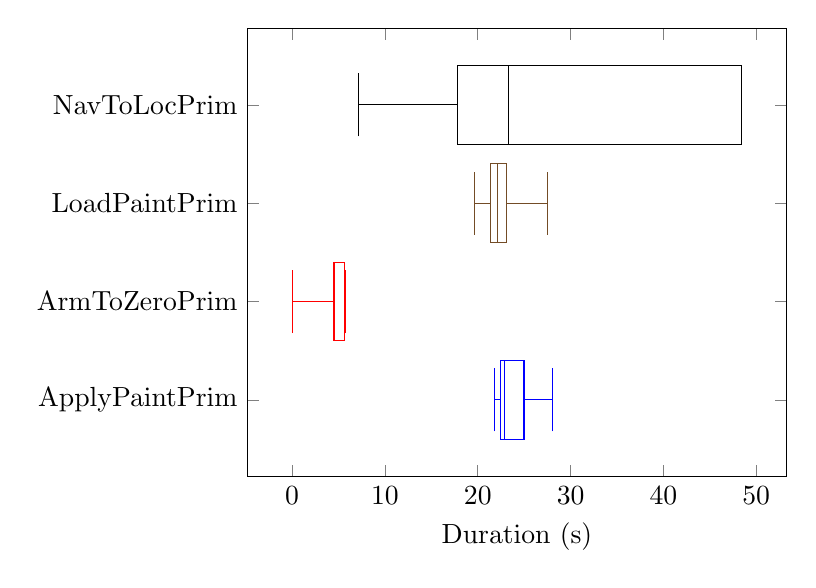
\begin{tikzpicture}
            \begin{axis}
            [
                xlabel={Duration (s)},
                ytick={1,2,3,4},
                yticklabels={ApplyPaintPrim, ArmToZeroPrim, LoadPaintPrim, NavToLocPrim}
            ]
            % ApplyPaintPrim
            \addplot+[
                boxplot prepared={
                    lower whisker=21.8184,
                    lower quartile=22.446975,
                    median=22.92375,
                    upper quartile=24.979375,
                    upper whisker=28.0878
                }
            ] coordinates {};
            % ArmToZeroPrim
            \addplot+[
                boxplot prepared={
                    lower whisker=0.0006,
                    lower quartile=4.49445,
                    median=4.5282,
                    upper quartile=5.6854,
                    upper whisker=5.7979
                }
            ] coordinates {};
            % LoadPaintPrim
            \addplot+[
                    boxplot prepared={
                    lower whisker=19.6744,
                    lower quartile=21.3819,
                    median=22.1672,
                    upper quartile=23.133,
                    upper whisker=27.5227
                }
            ] coordinates {};
            % NavToLocPrim
            \addplot+[
                    boxplot prepared={
                    lower whisker=7.1589,
                    lower quartile=17.8408,
                    median=23.3068,
                    upper quartile=48.4461,
                    upper whisker=48.4461,
                    %   upper whisker=398.6586
                }
            ] coordinates {};
            \end{axis}
        \end{tikzpicture}
    }
    \caption{A box plot of the execution time of each primitive skill. The upper whisker of the NavigateToLocationPrimitive plot has been truncated for visualization purposes -- this skill had a maximum recorded duration of \SI{398.6586}{\second}. The plot has been otherwise unaltered.}
    \label{fig:prim_time}
\end{figure}

Figure \ref{fig:prim_time} shows the execution time of each of the primitive skills across all simulations. The skills involving arm motion -- ApplyPaintPrimitive, ArmToZeroPrimitive, and LoadPaintPrimitive -- all show fairly consistent timings. This is due to the fact that, as they are currently designed, these motions are highly controlled and predictable. The ArmToZeroPrimitive skill simply returns the arm to a pre-defined position and, predictably, shows the lowest variation. The minimum recorded time for this skill is \SI{0.0006}{\second}, which is likely an erroneous value and may be considered an outlier. The execution times of the ApplyPaintPrimitive and LoadPaintPrimitive skills are very similar, as these skills cause the arm to perform essentially the same basic motion differing primarily in angle. Variation in the arm skill execution times is driven largely by the planning time of the MoveIt package.

The NavigateToLocationPrimitive skill exhibits a much wider range of execution time than the arm-based skills. Some variation is expected since the distance the robot must travel between locations and the obstacles it must navigate around will vary greatly and be unpredictable. The upper end of times taken by the NavigateToLocationPrimitive skill is noteworthy, however. As seen in figure \ref{fig:paintbot_room}, the room used during the simulations is not overly large and the obstacles are not overly complicated and thus does not warrant such high navigation times. These times are the result of several navigation problems that were observed.

First, the robot would occasionally take highly circuitous paths to arrive at its destination. In some instances, this was due to the fact that the TEB algorithm would plan routes through obstacles that had not yet been observed by the laser rangefinder. In such a scenario, the plan would have to be adjusted online to account for these obstacles as they came into the laser's field of view. In other instances, the TEB algorithm would fail to plan a shorter, more direct path and would instead settle on a longer path for unknown reasons. Second, the TEB algorithm would occasionally generate tight loops in the path near the goal that would cause the robot to make in-place or nearly-in-place rotations. This is likely due to both the curving, ``elastic band'' nature of the paths generated by TEB and the balance in the configuration of the algorithm between holonomic and non-holonomic motion. The last, and most predominant, of these problems were oscillations about the destination. Quite often, the TEB algorithm would generate very short, oscillating paths about the destination that could last upwards of several minutes. Navigations that took longer than approximately \SI{420}{\second} were manually terminated. Ten simulations were manually terminated for this reason. It is possible these oscillations are due to a combination of configured tolerances and SLAM update rate, but more investigation is required to confirm this.

\begin{table}
    \centering
    \begin{tabular}{|l|c c c c|}
        \hline
        & Min & Avg & Std Dev & Max \\
        \hline
        \hline
        $\bar{v}$ (m/s) & 0.0000 & 0.2264 & 0.0819 & 0.3473 \\
        \hline
        $\Delta x$ (m) & 0.0006 & 0.1326 & 0.0621 & 0.2174 \\
        \hline
        $\theta$ (rad) & 0.0016 & 0.0857 & 0.0209 & 0.1051 \\
        \hline
    \end{tabular}
    \caption{Metrics collected during the simulations for the velocity of the robot and the accuracy of its positioning.}
    \label{tbl:nav_metrics}
\end{table}

Table \ref{tbl:nav_metrics} shows the metrics collected about the robot's navigation. $\bar{v}$ is the robot's average velocity during the navigation skill, $\Delta x$ is the distance between the robot's destination and its true position at the completion of the navigation skill, and $\theta$ is the difference between the robot's goal heading and its true heading. The TEB algorithm was configured with a goal distance tolerance of \SI{0.2}{\meter}, a goal heading tolerance of \SI{0.1}{rad}, a maximum forward velocity of \SI{0.4}{\meter/\second}, and a maximum reverse velocity of \SI{0.2}{\meter/\second}. The distance and heading tolerances were selected for being the lowest values with which successful navigation paths were able to be generated a majority of the time.

The robot was able to navigate within the defined tolerances the vast majority of the time, as expressed in table \ref{tbl:nav_metrics}. However, these tolerances are not likely to be acceptable for many construction tasks that require precise positioning. If TEB continues to be used for this robot into the future, further work must be done to determine how to reduce these tolerances. A potential solution that could be made is the addition of a secondary fine-grained navigation skill. This skill would activate after the robot has navigated to within the coarse-grained tolerances of TEB and would make more explicit, finer adjustments to the robot's position. The robot's generally low average velocity during the NavigateToLocationPrimitive skill (approximately $57\%$ of its maximum) is largely due the excess movement resulting from the oscillations and loops discussed earlier.

\subsection{Planning Test Results} \label{sec:results_plan}
Each planning test scenario specified a single length of wall to be painted a number of colors. The wall varied between \SI{1}{m} and \SI{5}{m} in length in \SI{1}{m} increments, resulting in a range of $5-24$ wall sections. The number of colors per scenario varied between $1$ and $3$. The length of wall was divided evenly into segments to match the number of paints and a paint was assigned to each one. The scene was generated using the Scene Generator program discussed in section \ref{sec:interaction}. Each scenario was simulated $5$ times for a total of $75$ simulations ($5$ wall lengths $\times$ $3$ paints $\times$ $5$ runs).

\begin{figure}
    \centering
    \resizebox{0.75\linewidth}{!}{
        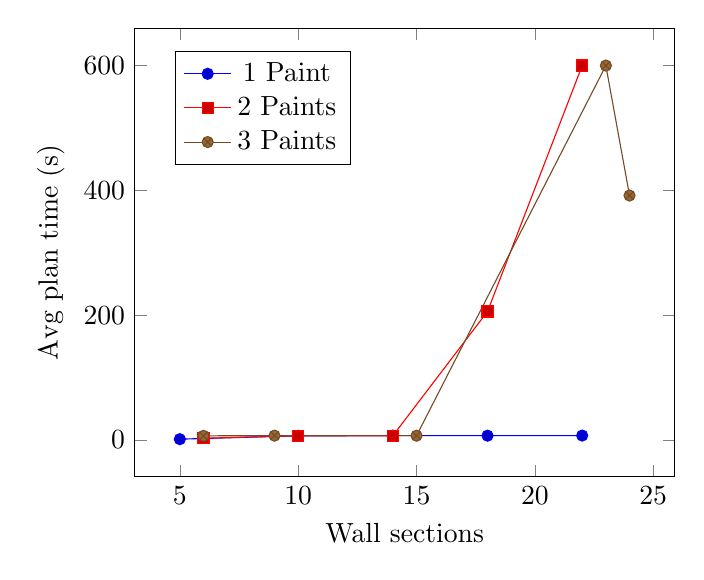
\begin{tikzpicture}
            \begin{axis}
            [
                xlabel={Wall sections},
                ylabel={Avg plan time (s)},
                legend style={at={(0.40,0.95)}}
            ]
            % 1 paint
            \addplot coordinates {(5,1.258) (10,6.705) (14,6.945) (18,6.872) (22,7.051)};
            \addlegendentry{1 Paint}
            % 2 paints
            \addplot coordinates {(6,2.712) (10,6.725) (14,6.760) (18,205.952) (22,600.000)};
            \addlegendentry{2 Paints}
            % 3 paints
            \addplot coordinates {(6,6.595) (9,6.897) (15,6.838) (23,600.000) (24,391.750)};
            \addlegendentry{3 Paints}
            \end{axis}
        \end{tikzpicture}
    }
    \caption{Time taken by the TFD planner to generate plans for a number of paints and an increasing number of wall sections.}
    \label{fig:plan_time}
\end{figure}

Figure \ref{fig:plan_time} shows the planning times for each paint as a function of the number of wall sections. The planning time for a single paint color remained stable at approximately \SI{6.5}{\second}-\SI{7}{\second} across the entire range of wall sections tested for. However, adding additional colors to the scene resulted in erratic and non-obvious changes in the planning time. An extremely sharp increase was observed when the scene contained $2$ or more paints and more than approximately $15$ wall sections. The TFD planner was configured with a time limit of \SI{600}{\second}, after which planning would fail. This happened for two of the scenarios. Curiously, The scenario containing $3$ paints and $24$ wall sections consistently required less planning time than the two less complex scenarios that failed. I have yet to determine the reason for this. 

The times for the $2$ and $3$ paint scenarios are generally too high for practical use and will need to be addressed in the future. The $1$ paint times are adequate for operation inside of a relatively static environment, such as an off-hours construction site where the basic conditions of tasks are unlikely to change. In such a case, online replanning would not be necessary. However, in more dynamic environments where conditions may change rapidly, such as equipment being repositioned by coworkers or new events rendering some tasks impossible, \SI{6.5}{\second}-\SI{7}{\second} may become prohibitively expensive. It should be noted that navigation and obstacle avoidance are performed online and are not part of the task planning process.
\section{Conclusion and Future Work} \label{sec:conclusion}
This paper presents a functional proof of concept for a small, mobile, autonomous, and extensible construction robotics platform. The platform is based on ROS and extended the well known and well supported ROS-based packages to manage the task planning, arm motion control, and navigation of the robot. The simulations demonstrate that the concept of such this feasible robot platform could satisfy the performance requirements of construction industry. Though the only task demonstrated was wall painting, nothing in the design of the platform prohibits it from being expanded to work for arbitrary tasks. %The use of a general purpose task planning framework, such as SkiROS, ensures this. 
The painting and navigation skills were shown to be able to interact with one another and allow for complex and dynamic behaviors. However, there is still much work to be done and room for growth.

The most serious issues with the platform, as designed thus far, are with some of the algorithms chosen. In particular, the TEB algorithm~\cite{rosmann2012trajectory} has been shown to have difficulty planning paths that successfully direct the robot to its destination once in close proximity to the destination, even with holonomic motion. The TFD algorithm~\cite{eyerich2009using} has shown irregular performance when planning painting tasks for a small number of entities. These issues are a high priority and should be resolved by either correcting the configuration of the algorithms or replacing the algorithms altogether.

Furthermore, the development of the robot should be continued using physical hardware. While software simulation is beneficial for rapid prototyping, it is a radically different environment from hardware in the physical world. The move to physical hardware will bring with it many changes. First, the size of the robot will need to be updated. The simulated YouBot is rather small -- the arm only vertically reaches \SI{0.655}{\meter} fully extended. While this has been sufficient for testing the general concepts motivating this project, it limits the robot's practical effectiveness. Second, a manipulator arm with more or less than the $5$ degrees of freedom tested in this project will greatly impact the sorts of actions that can be performed. Finally, the drive system (i.e. holonomic vs. non-holonomic) will dictate which navigation algorithms are viable.

Moreover, once the hardware to be used is more well understood, a system will need to be devised that allows the robot to utilize a wide variety of tools and equipment. This could mean grasping and manipulating tools with a gripper or a modular system that allows the robot to swap tool attachments on its arm. Additionally, the sensor suite on the robot will need to be expanded. The single front-mounted laser rangefinder present on the simulated YouBot is sufficient only for basic navigation. A robot working in a construction zone with dangerous tools and materials requires much greater situational awareness than represented here. Examples include adding more rangefinder devices with greater coverage area around the robot and one or more cameras for object recognition.

In addition, Building Information Modeling (BIM) is a process used in the construction industry for representing and managing construction requirements. Many popular construction planning software tools output files containing BIM data. This information has some conceptual similarities to languages and formats used to encode information in computer science, such as OWL and PDDL. It should be possible to bridge this gap and convert from one domain to the other. An application (such as the Scene Generator) could take BIM data as input and translate it into a format that can be used by planning algorithms. Incorporating BIM into the operation of the robot in this way could help to greatly increase both the value provided by the platform and its adoption rate by the construction industry.

%\printbibliography
\bibliographystyle{IEEEtran}
\bibliography{bibliography}

%\appendix

\section{Skill PDDL} \label{app:skill_pddl}
\begin{verbatim}
(define (domain untitled)
(:requirements :typing :fluents :universal-preconditions)
(:types 
    paintbot:WallSection paintbot:Paint rparts:ArmDevice
            sumo:Agent skiros:Location paintbot:PaintTray - thing
    rparts:ArmDevice paintbot:WallSection - paintbot:hasColorx
    paintbot:WallSection skiros:Location paintbot:PaintTray - skiros:aty
)
(:predicates 
    (paintbot:targetColor ?x - paintbot:WallSection  ?y - paintbot:Paint )
    (paintbot:hasColor ?x - paintbot:hasColorx  ?y - paintbot:Paint )
    (skiros:at ?x - sumo:Agent  ?y - skiros:aty )
    (Painted ?x - paintbot:WallSection )
    (skiros:contain ?x - paintbot:PaintTray  ?y - paintbot:Paint )
)
(:functions
)
(:durative-action loadpaint
    :parameters (?Paint - paintbot:Paint
        ?Tray - paintbot:PaintTray
        ?Arm - rparts:ArmDevice
        ?Robot - sumo:Agent )
    :duration (= ?duration 1)
    :condition (and
        (at start (skiros:contain ?Tray ?Paint))
        (at start (skiros:at ?Robot ?Tray))
        (over all (skiros:at ?Robot ?Tray))
    )
    :effect (and
        (at end (paintbot:hasColor ?Arm ?Paint))
    )
)

(:durative-action applypaint
    :parameters (?Wall - paintbot:WallSection
        ?Paint - paintbot:Paint
        ?Arm - rparts:ArmDevice
        ?Robot - sumo:Agent )
    :duration (= ?duration 1)
    :condition (and
        (at start (paintbot:targetColor ?Wall ?Paint))
        (at start (paintbot:hasColor ?Arm ?Paint))
        (at start (skiros:at ?Robot ?Wall))
        (over all (paintbot:hasColor ?Arm ?Paint))
        (over all (skiros:at ?Robot ?Wall))
    )
    :effect (and
        (at end (paintbot:hasColor ?Wall ?Paint))
        (at end (Painted ?Wall))
    )
)

(:durative-action navigatetolocation
    :parameters (?Start - skiros:Location
        ?Destination - skiros:Location
        ?Robot - sumo:Agent )
    :duration (= ?duration 1)
    :condition (and
        (at start (skiros:at ?Robot ?Start))
        (at start (not (skiros:at ?Robot ?Destination)))
    )
    :effect (and
        (at start (not (skiros:at ?Robot ?Start)))
        (at start (skiros:at ?Robot ?Destination))
    )
)

)
\end{verbatim}

\end{document}
